%!Tex Root = ../main.tex
% ./Packete.tex
% ./Design.tex
% ./Deklarationen.tex
% ./Vorbereitung.tex
% ./Aufgabe1.tex
% ./Aufgabe2.tex
% ./Aufgabe4.tex
% ./Appendix.tex

\section{Aufgabe 3}

\setcounter{exercise}{1}

% \begin{frame}[allowframebreaks]{Aufgabe \thesection}{Zustandsdiagramme, Mealy-Automaten}
%
% \end{frame}

    % \begin{frame}{Aufgabe 3}{}
    %     \begin{block}{Aufgabe}
    %         Zeichne Zustandsdiagramm von:\\
    %         Incrementer einer Binärzahl als Mealy-Atomat:
    %         \begin{itemize}
    %             \item niedrigstwertiges Bit wird zuerst gelesen
    %             \item auf das höchstwertige Bit folgt $\#\#$
    %             \item das erste $\#$ wird durch das Überlauf-Bit ersetzt, das zweite bleibt stehen
    %             \item Symbole nach der Endmarkierung sollen durch $\#$ ersetzt werden
    %         \end{itemize}
    %     \end{block}
    % \end{frame}

    \begin{frame}{Aufgabe \thesection}{Zustandsdiagramme, Mealy-Automaten}
        \begin{solutionnoinc}
            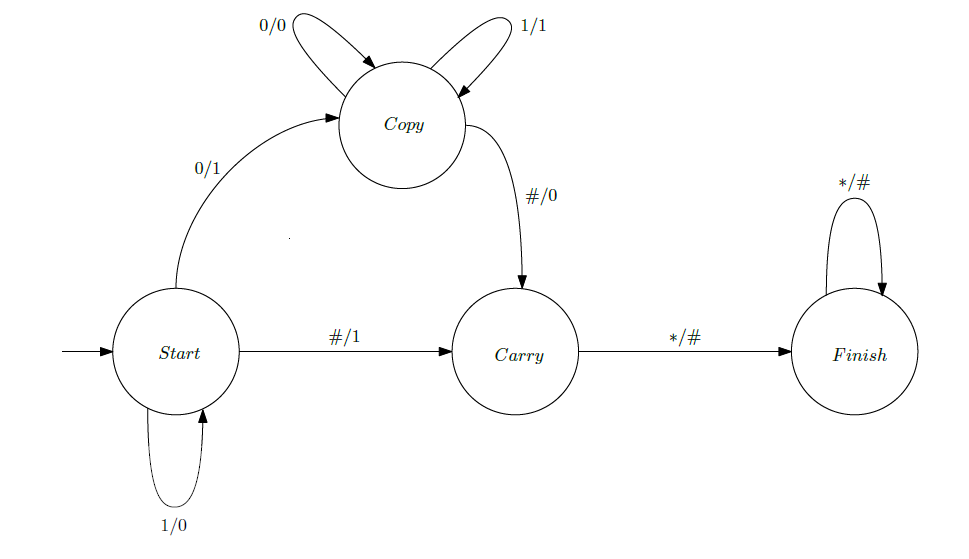
\includegraphics[height=0.5\paperheight, center]{./figures/Mealy-Increment.png}
        \end{solutionnoinc}
    \end{frame}
